\documentclass[12pt,a4paper]{article}
\usepackage{cite}
\usepackage{fullpage}
\usepackage{indentfirst}
\usepackage{parskip}
\usepackage{amsmath}
\usepackage{hyperref}
\usepackage{bm}
\usepackage{enumerate}
\usepackage{enumitem}
\usepackage{graphicx}
\usepackage{booktabs}
\usepackage{url}
\usepackage{textcomp}
\usepackage[UTF8]{ctex}

\begin{document}
\setlength{\parindent}{2em}

\pdfbookmark[0]{Front page}{label:frontpage}%
\begin{titlepage}
  \noindent%
  \begin{tabular}{@{}p{\textwidth}@{}}
    \toprule[2pt]
    \midrule
    \vspace{0.2cm}\\
    \begin{center}
    \Huge{\textbf{
      基于AODV的支付通道网络\\路由协议 \\[8pt]
    }}
    \end{center}
    \begin{center}
      \Large{
        分布式计算课程主题报告
      }
    \end{center}
    \vspace{0.2cm}\\
    \midrule
    \toprule[2pt]
  \end{tabular}
  \vspace{5 cm}
  \begin{center}
    {\Large
      第15组
    }\\
    \vspace{0.2cm}
    {\Large
      1831605 \quad 刘诗洋 \\[5pt]
      1831606 \quad 陆思远 \\[5pt]
      1831607 \quad 余\quad豪 \\[5pt]
    }
  \end{center}
  \vfill
  \begin{center}
    {\Large
      同济大学\\[5pt]
      软件学院\\[5pt]
    }
  \end{center}
\end{titlepage}
\clearpage

\tableofcontents
\clearpage

\section{概述}
这篇报告是我们以论文\cite{hoenisch2018aodv}为基础,在较为充分的文献查阅及原理探究后,对支付通道网络及其路由协议做的内容梳理。我们从区块链的一大应用:加密货币开始,介绍其现状及共有问题。为了解决这些问题,研究者们提出了链下的支付网络,也即支付通道网络(Payment Channel Network, PCN),其中闪电网络(Lightning Network, LN)是较为突出的代表。但以主动式路由为路由协议的LN存在一些固有局限,为了发挥PCNs的潜力,研究者提出了以AODV(Ad-hoc On-demand Distance Vector)为基础的被动式路由协议,以期有效地解决问题。基于以上问题和解决方案,我们的报告内容也将按这一顺序展开,具体为:
\begin{itemize}
	\item 区块链及其应用的发展、愿景及问题;
	\item 闪电网络;
	\item 支付通道网络的特性、问题及需求;
	\item 路由协议及其种类简介;
	\item 基于AODV的路由协议及算法详述;
	\item 网络及协议性能评价;
	\item 总结与展望。
\end{itemize}

\section{区块链的发展、目标与问题}
随着比特币\cite{nakamoto2008bitcoin}以及其他诸多电子加密货币的出现,区块链一词逐渐被人们所知。作为比特币背后的技术基础,区块链可被认为是所有比特币交易的公共分类账簿。\cite{swan2015blockchain}由于它的去信任化机制,用户可以信任这一系统,并将所有的交易记录在去中心化的节点上;而非像传统做法一样,由中心化的第三方机构来维护。区块链真正的独特技术在于它不需要用户去信任任何的中心机构,而是通过算法的自我监督,任何恶意欺骗系统的企图都将被拒绝。区块链的潜在优势不仅仅体现在金融上,在政府管理、人道主义、社会和科学领域都有可能发挥作用。随着物联网及5G通信时代的到来,机器间的经济交易也将急剧增长。Gartner\cite{iot_economic}估计,到2020年,全球物联网将包括260亿台设备并产生1.9万亿美元的经济规模。管理这些设备之间的交易需要相应的加密货币,进而形成货币互联网。此外,相互连接的设备之间的小额支付可能会发展成为经济的一个新层次\cite{new_layer_economy}。

区块链旨在建立一个去中心化的网络,然而,随之而来的是一些问题\cite{blockchain_problem}。一个主要问题是,随着区块链网络信息量日益增大,整个网络变得拥挤,交易时间和成本飙升。就比特币来说,一次交易经常需要经过6次区块节点确认,平均耗时超过60分钟;另外,高昂的交易费用也使得小额交易望而却步。除此之外,研究人员发现比特币交易中的数据块可能隐藏着一些非法内容(儿童色情信息等),这些图像或视频文件由于被加密,便与合法的比特币数据混在一起,难以发现。此外,由于比特币的奖励机制,比特币矿工在维护和挖掘比特币时将会得到比特币奖励,但伴随着的是高昂的计算硬件和电力成本。随着维护和挖掘难度增大和比特币的价格变动,成本和收益之间的平衡难以维持,不过目前为止还没有出现网络的崩溃。

针对第一个问题,研究者们设想不在区块链上解决每笔交易,而是将部分交易转移到链下,允许交易双方直接接触。通过自身直接跟踪支付流程,双方即可避免链上交易的高耗时及高费用。若用户存在余额的争议或是有一方无响应,则双方可提供最新的资产负债表并在区块链上解决。在此类解决方案中,闪电网络(Lightning Network, LN)是较为突出的代表,它提出了一个脱链支付通道覆盖网络(PCN),下面我们将详细介绍LN相关内容。


\begin{figure}[htb]
\centering
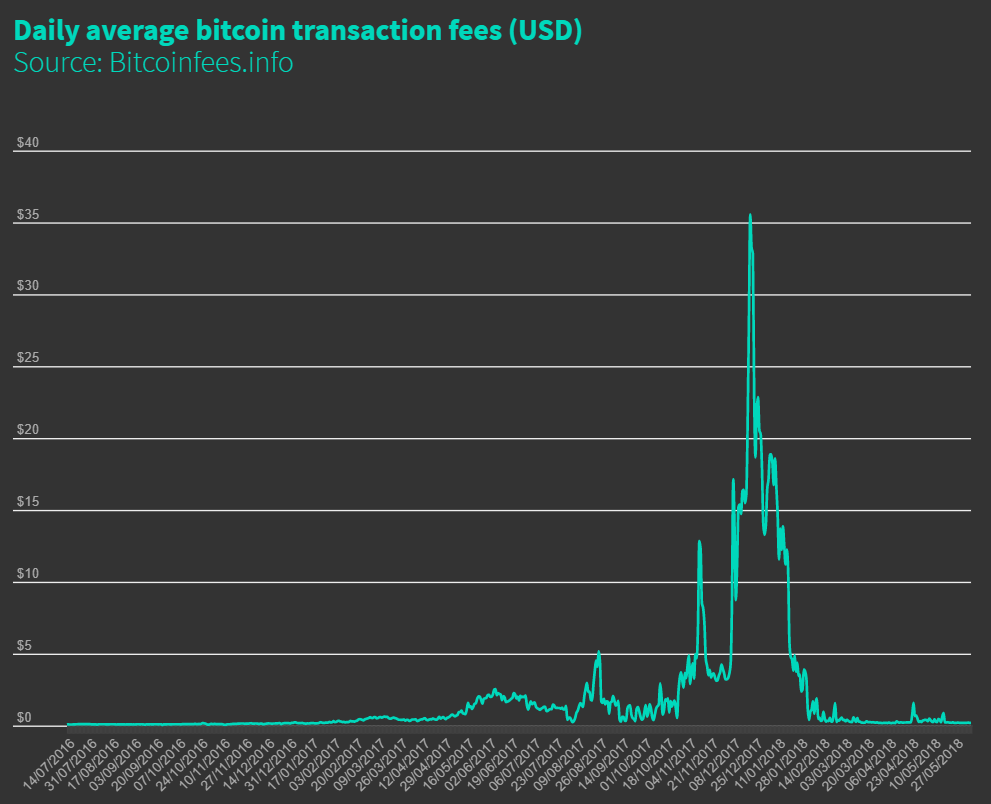
\includegraphics[width=7cm]{fee}
\caption{比特币日均每笔交易费用(美元)}
\end{figure}

\begin{figure}[htb]
\centering
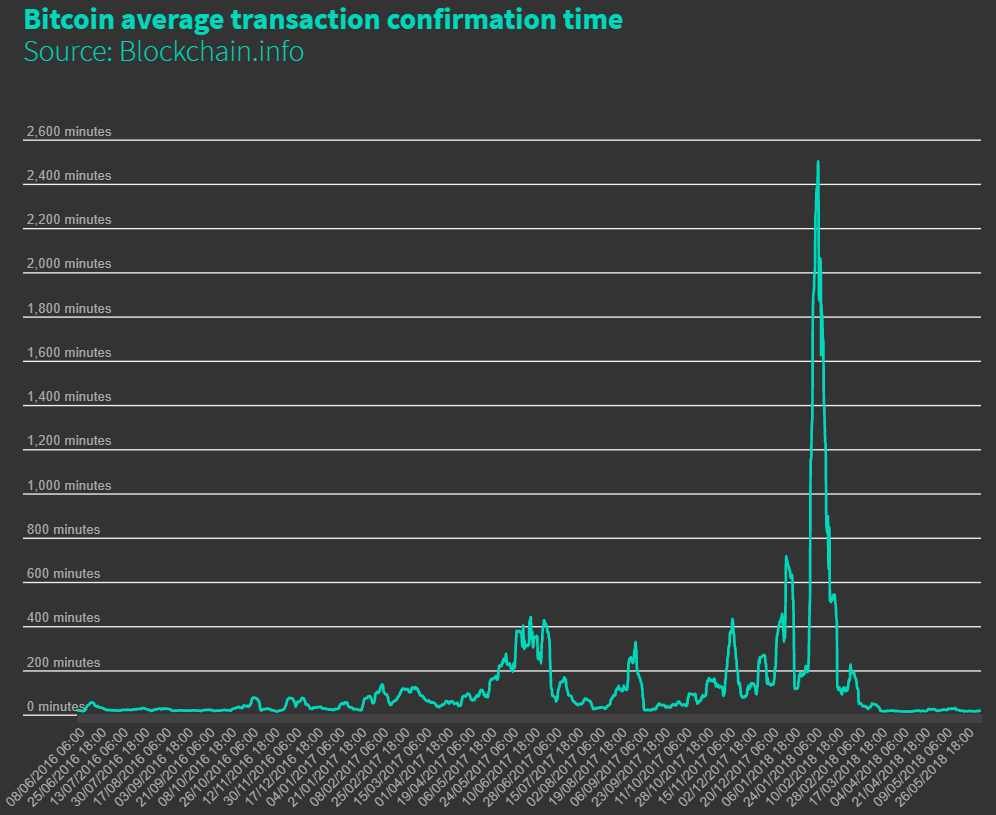
\includegraphics[width=7cm]{time}
\caption{比特币日均每笔交易确认时间(分钟)}
\end{figure}

\clearpage

\section{闪电网络}
\subsection{定义与特性}
闪电网络\cite{poon2016bitcoin}是一种轻量级的软件解决方案,用于扩展公共区块链与加密货币的互操作性。它是一个去中心化的系统,使得即时、大量的小额支付成为可能,且消除了将资金委托给受信任的第三方的风险。闪电网络最初由MIT媒体实验室针对比特币进行研发,但可以拓展应用于所有类似于比特币的区块链。具体来说,闪电网络的功能特性有如下四点。

\begin{enumerate}
	\item 即时支付。比特币将交易聚合成块,每10分钟进行一次。人们普遍认为,比特币在6次区块(耗时约1小时)确认后将被认为是安全的。显然这种确认时间不适合许多场景下的即时交易。而在闪电网络中,支付不需要经由区块确认,可以达到即时性和原子性。因此,闪电网络可以被广泛应用于销售终端、用户设备间交易以及其他需要即时支付的场景。

	\item 小额支付。闪电网络可以使得单笔交易额降至0.00000001比特币(低于0.01美分),且无需承担托管风险,而比特币的链上交易单笔最少数额要比这一值高数百倍。由于比特币单笔交易收费固定(远高于0.01美分),所以在链上进行小额交易是不切实际的。通过闪电网络,小额支付便可以进行,新的市场也得以开辟。


	\item 可扩展性。闪电网络将许多微支付通道连接成为网络,利用这个网络,比特币区块链在一台现代个人电脑上就可每天处理数十亿笔交易。大量的资金可以通过去中心化的方式在给定的交易通道内进行转移,这些通道并非在比特币之上建立独立的信任网络,每一笔经由通道的交易都是真实的比特币交易。

	\item 跨链交易。通过闪电网络,跨链间的原子性交易可以在链下实时发生,只要异构的区块链满足一致性准则。也即只要各个区块链支持相同的哈希函数,就有可能不在受信任的第三方托管下进行跨链交易。
\end{enumerate}

\subsection{关键技术}
闪电网络依赖于区块链的底层技术,通过使用原生的智能契约脚本,并进行真实的比特币交易,就可以创建一个安全的参与者网络,并以高容量和高速度进行交易。下面介绍闪电网络的两个核心概念:RSMC和HTLC。

\textbf{RSMC} (Recoverable Sequence Maturity Contract),即“可撤销的顺序成熟度合同”。首先假定交易双方之间存在一个微支付通道(资金池)。交易双方先预存一部分资金到微支付通道里,初始情况下双方的分配方案等于预存的金额。每次发生交易,需要对交易后产生资金分配结果共同进行确认,同时签字把旧版本的分配方案作废掉。任何一方需要提现时,可以将他手里双方签署过的交易结果写到区块链网络中,从而被确认。从这个过程中可以可以看到,只有在提现时候才需要通过区块链。

任何一个版本的方案都需要经过双方的签名认证才合法。任何一方在任何时候都可以提出提现,提现时需要提供一个双方都签名过的资金分配方案(意味着肯定是某次交易后的结果,被双方确认过,但未必是最新的结果)。在一定时间内,如果另外一方拿出证明表明这个方案其实之前被作废了(非最新的交易结果),则资金罚没给质疑方;否则按照提出方的结果进行分配。罚没机制可以确保了没人会故意拿一个旧的交易结果来提现。另外,即使双方都确认了某次提现,首先提出提现一方的资金到账时间要晚于对方,这就鼓励大家尽量都在链外完成交易。通过 RSMC,可以实现大量中间交易发生在链外。

下面举例说明RSMC的详细过程。假设Alice和Bob需要进行交易,那么在微支付通道建立时,双方必须有一定的资金沉淀在该通道上,我们假设目前通道中资金为:Alice: 0.4, Bob: 0.6,这样预存到通道的资金共有1.0 BTC,其中Alice拥有0.4 BTC,Bob拥有0.6 BTC。而支付通道的设立会记录在比特币的区块链上。某次,Bob决定向Alice支付0.1 BTC。在双方都签字认可的情况,链下支付通道的最新余额分配方案将变为{Alice:0.5, Bob:0.5},而且双方需要同时签字同意作废前一版本的余额分配方案{Alice:0.4, Bob:0.6},这样Alice就实际获得了0.5 BTC的控制权。

若Alice考虑到以后还会和Bob进行交易,那么她可以无需提取现在属于她的0.5 BTC,也无需在比特币区块链上更新已有变动的余额分配方案,因为若他们再次进行交易(如Alice向Bob支付0.2BTC)的话,他们仍然只需在链下对目的的余额分配方案达成一致,并设法作废前一版本的余额分配方案就行了。若Alice不打算再次和Bob进行交易并想动用通道的资金,她可以向区块链出示双方签字的余额分配方案。如果在规定时间内Bob未提出异议,区块链则会终止双方的支付通道并将资金按协议转入各自预先设立的提现地址。如果Bob在规定时间内提交证据证明Alice提交的是一个双方已同意作废的余额分配方案,那么Alice的资金将被罚没并给到Bob。

\textbf{HTLC} (Hashed Timelock Contract),即“哈希的带时钟的合约”,用于保证限时转账。通过智能合约,双方约定转账方先冻结一笔钱,并提供一个哈希值,如果在一定时间内有人能提出一个字符串,使得它哈希后的值跟已知值匹配(实际上意味着转账方授权了接收方来提现),则这笔钱转给接收方。

依然使用示例来说明该过程。如图所示,Alice(A)想给Darcy(D)发送0.05 BTC,但Alice和Darcy之间并没有微支付通道。但这没关系,闪电网络为Alice匹配了一条经过Bob(B)、Cady(C)到达Darcy的支付路径,该路径由Alice-Bob, Bob-Cady和Cady-Darcy这样三个微支付通道接力而成。Darcy生成一个哈希值$R$并将$Hash(R)$发送给Alice,Alice不需要知道$R$。$R$和$Hash(R)$的作用类似于钥匙和锁,只有匹配在一起才可开锁。Alice和Bob商定一个HTLC合约:只要Bob能在3天内向Alice出示正确的$R$,Alice会支付Bob 0.052 BTC;如果Bob做不到这点,这笔钱3天后自动退还Alice。同样地,Bob和Cady商定一个HTLC合约:只要Cady能在2天内向Bob出示哈希正确的$R$,Bob会支付Cady 0.051 BTC;如果Cady做不到这点,这笔钱到期自动退还Bob。最后,Cady和Darcy商定一个HTLC合约:只要Darcy能在1天内向Cady出示哈希正确的$R$,Cady会支付Darcy 0.05 BTC;如果Darcy做不到这点,这笔钱到期自动退还Cady。

方案确定好后,Darcy及时向Cady披露R并拿到0.05 BTC;现在Cady知道了$R$,她可以向Bob出示密码$R$并拿到0.051 BTC(差额部分的0.001 BTC成了Cady的佣金);Bob知道$R$后当然会向Alice出示并拿到他的那份 0.052 BTC,差额部分的 0.001 BTC成了Bob的佣金。大家可以看到,最终的结果是Alice通过闪电网络安全地向Darcy支付了 0.05 BTC,所付出的代价仅仅是支付给Bob和Cady(节点)的 0.002 BTC“过路费”(佣金)。

\begin{figure}[htb]
\centering
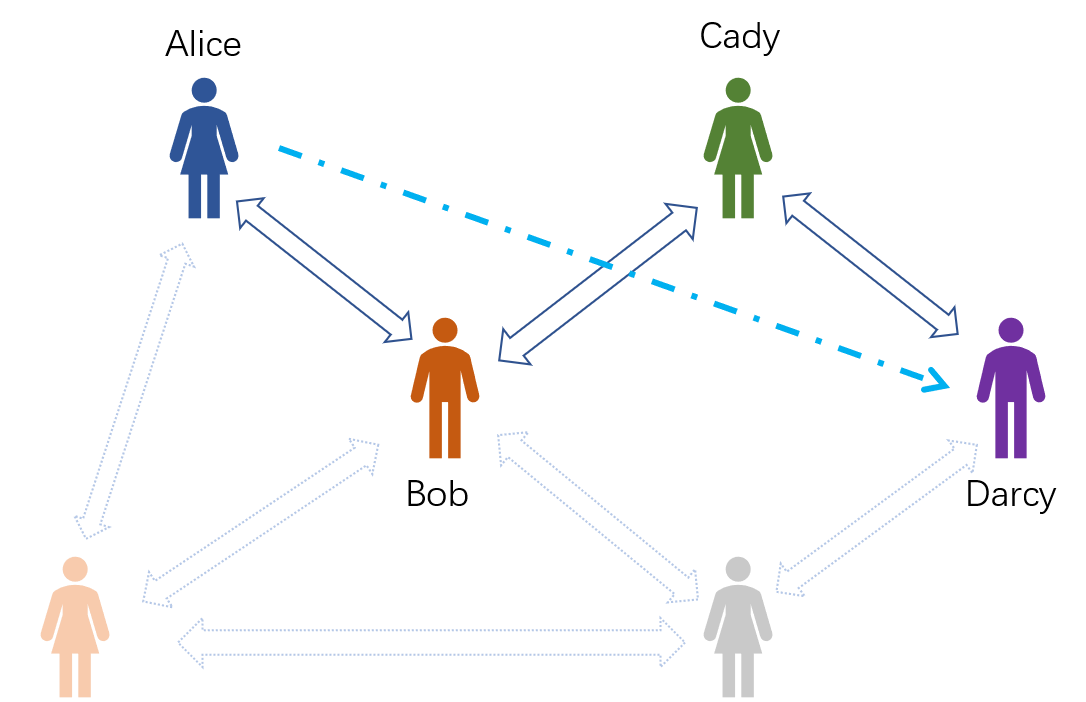
\includegraphics[width=9cm]{channels}
\caption{闪电网络微支付通道}
\end{figure}

\subsection{小结}
闪电网络的理念就是引入了一个类似于第三方中介且仅适用于高频次、小额交易的微支付通道。交易双方在这个微通道中必须先预存一定数量的保证金,而由区块链产生的智能合约(资金分配方案)进行监督评判。闪电网络中的所有交易动作都是发生在区块链之外,只有当需要提现时,才会将最终的交易结果写到区块链网络中并被最终确认。这大大降低了比特币区块链上的交易压力。

其中,RSMC 保障了两个人之间的直接交易可以在链下完成,HTLC 保障了任意两个人之间的转账都可以通过一条“支付”通道来完成。闪电网络整合这两种机制,就可以实现任意两个人之间的交易都在链下完成了。智能合约起到了中介的重要角色,而区块链网络则确保最终的交易结果被确认。

\section{路由协议}
\subsection{闪电网络中的通道寻优}
如第三部分所述,当交易双方之间没有直连的微支付通道时,需要将若干个支付通道连接,方可进行交易。在这个过程中,如何在发送方和接收方之间寻找到最优(或可接受)的路由通道将是一个挑战。在这个特定网络里,路由协议需要考虑路由费用、汇率以及可靠性等指标,使之可被接受。闪电网络使用主动式的路由协议,每个节点通过网络广播其邻居的信息(例如,广播通过网络连接的节点信息)。每个节点都具有关于网络拓扑的路由表,然而,这样做的缺点是在建立路由前需要发送大量信息。而且,在这样的基础上,我们只能获知通道的金融信息,而不包括整个资金的分布,也即想要获知哪一方拥有多少金额,只能寻求与比特币的区块链。显然,广播全局的拓扑信息耗费巨大,且会产生扩展限制,这在跨链网络的情况下尤为严重。因此,研究者们寻求设计其他路由算法,以求突破这一限制,下面先简要介绍主要的几种路由协议。
\subsection{路由协议的类型}
路由指电子通信网络通过确定网络中的路径,并通过这种路径高效快速地将一个信息单元从A点发送到B点的能力\cite{medhi2017network}。而路由协议则是描述具体的寻路算法,使得整个网络通信更加高效且可靠。由于目前研究者对PCN的研究较少,所以我们将目光移向移动自主网络(MANET, Mobile Ad hoc Network)。MANET是指能够自主配置的可移动节点的网络集合,集合内的节点可以自由移动,并可在任何时候连接到不同的节点。与PCN类似,MANET内的节点的出现和消失并不规律,且通道的平衡经常变化。在MANET里,路由协议可以分为五大类型:主动协议、被动协议、混合协议、分层协议和基于协调的协议。

主动协议\cite{Alslaim2014}使用链路状态路由算法,每个节点都会维护一到多个包含路由到网络中其他所有节点的路由表。所有的节点持续更新它们的路由表来维护最新的网络视图。这种路由协议适用于静态场景,两个较为著名的协议为DSDV(Destination-Sequenced Distance Vector routing)和WRP(Wireless Routing Protocol)\cite{Murthy1996}。

被动协议减少了主动协议中存在的开销。它使用距离向量路由算法,并且仅当一个节点启动路由发现过程请求指定目的地时,才建立到该目的地的路由。在信息到达目的地后,以及这条路由不再需要前,该路由持续有效。比较典型的协议有AODV(Ad-hoc On-demand Distance Vector)和DSR(Dynamic Source Routing)\cite{Johnson, Perkins1999}。

混合协议将主动协议与被动协议混合,在此种协议下,每个节点主动维护一定区域内的路由信息表,若目的地超出了这一范围,则使用路由发现过程。混合协议的代表有ZRP(Zone Routing Protocol)、EIGRP(Enhanced Interior Gateway Routing Protocol)。

下面用表格来对比上述三类协议的异同。

\begin{table}[htb]
\renewcommand\arraystretch{1.2}
\caption{主动协议、被动协议与混合协议异同比较}
\centering
\begin{tabular}{l l l l}
\\
\hline
\hline
~ \textbf{特征} ~ & ~ \textbf{被动协议} ~ & ~ \textbf{主动协议} ~ & ~ \textbf{混合协议} \\[6pt]
\hline
路由结构  & 扁平结构 & 扁平及分层结构 & 分层结构 \\[6pt]
\hline
路由获得 & 按需获取 & 表驱动 & 二者混合
\\[6pt]
\hline
路由开销 & 低 & 高 & 中等
\\[6pt]
\hline
延迟 & 高(由于泛洪) & 低(由于主动路由) & 中等
\\[6pt]
\hline
可扩展性 & 不适用于大型网络 & 低 & 适用于大型网络
\\[6pt]
\hline
路由信息 & 需要时可用 & 始终可用 & 介于二者间
\\[6pt]
\hline
定期更新 & 不需要 & 网络改变时即需更新 & 需要
\\[6pt]
\hline
移动性 & 路径维护 & 定期更新 & 二者结合
\\[6pt]
\hline
存储需求 & 低 & 高 & 中
\\[6pt]
\hline
带宽需求 & 低 & 高 & 中
\\[6pt]
\hline
电力需求 & 低 & 高 & 中
\\[6pt]
\hline
\hline
\end{tabular}
\end{table}

而分层路由和基于协作路由的协议是通过位置相关的地址来进行路由的,用基于位置的算法取代了泛洪传播消息。前者的典型例子有LANMAR\cite{Guangyu}和L+\cite{mitton2005distributed},后者的例子有GPSR\cite{Karp2000}和BVR\cite{fonseca2005beacon}。

上述路由协议大多数都是为MANET设计,与PCN的需求还有些不同。例如,由于PCN涉及到资金锁定、汇率变动、节点费用变动等,一个路由响应会改变网络的状态,使得先前的通道不可用。但研究者们依然可以从MANET路由协议中获取一些灵感。

\subsection{Flare协议}
Prihodko等人提出了针对闪电网络的路由协议Flare\cite{prihodko2016flare}。Flare协议作为混合式协议,由主动和被动两个部分,提出该协议主要基于闪电网络的信息可以被分为两类:
\begin{itemize}
	\item 缓慢变化或静态的信息(节点之间的支付通道);
	\item 快速变化或动态的信息(节点状态、支付渠道内资金分配、使用渠道费用等)。
\end{itemize}

因此,主动(按确定的时间周期或按受限的泛洪方式)收集闪电网络中刚打开或关闭的支付通道是有意义的,这部分信息是闪电网络节点的兴趣内容;而主动收集会快速变化的信息是没有意义的,因为它们在不可预测的时间内都可能发生改变。

下图是Flare协议算法的概要架构。图中路由模块对应的便是闪电网络的业务逻辑。该模块的目标是提供一个或多个支付路径(如LN节点列表)发送给指定的收件人。为了实现这一目标,节点点通过交互来获取网络信息。获取方式包括主动(通过发现节点的邻居和信标)以及被动(通过选择和排序候选路线)。收集到的信息被放置到节点的路由表中,路由表用于处理来自节点操作者和其他节点的请求。

\begin{figure}[htb]
\centering
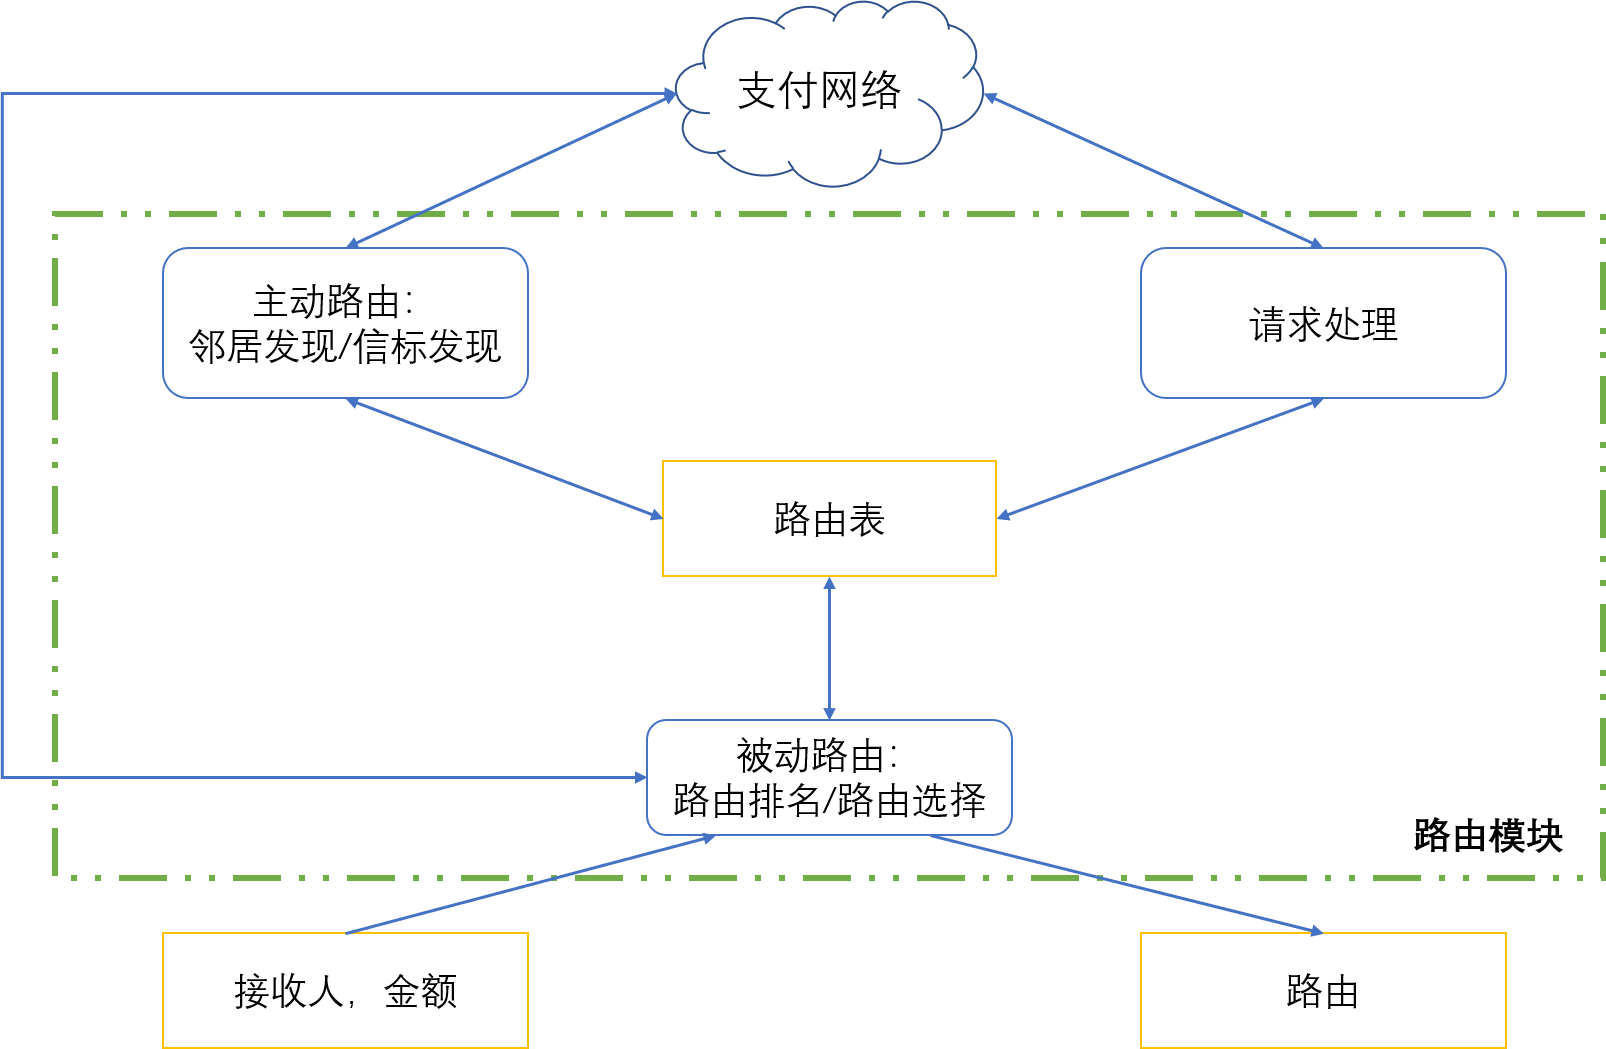
\includegraphics[width=9cm]{high_level_flare}
\caption{Flare协议抽象架构}
\end{figure}

与Flare不同,Hoenisch等人提出了另一种解决方案\cite{hoenisch2018aodv}。他们认为Flare专注于发送节点的安全性和审查阻力,而\cite{hoenisch2018aodv}关注每个中间节点的自主性。每个节点不应被迫将支付转发到某个特定的方向,这个决策是从经济的角度出发的。他们假设节点主要关注利润最大化,因此更有可能选择保证高利润的路线。这一基于AODV协议的算法是本篇报告所要阐述的重点,将在下文展开。
\subsection{PCN的基本假设}
在针对PCN提出路由算法前,先提出对PCN的基本假设:网络处于持续变化(网络的变化发生得比节点发出支付操作更频繁)。网络的持续变化源自于以下几个情况:
\begin{enumerate}
	\item 通道频繁更改:如付款前有效的路由在付款后不一定有效。
	\item 费用可能会经常变动:每个中间节点在转发支付时可以收取任意数量的费用。该节点可以定期更新该费用,以保持其通道平衡。例如,如果一个通道的流动性有耗尽的风险,节点在通过该通道转送付款时可能会收取更高的费用。
	\item 汇率可能变化很快:两个区块链之间的节点需要频繁地调整汇率;否则,这个节点可能有赔钱的风险。
	\item 节点可能在一段时间内处于脱机状态(或不可到达状态):
	由于在支付过程中节点需要接受和转发支付请求,所以节点基本是随时在线的,但如果中间节点离线,网络应该相应地进行调整。
\end{enumerate}

\subsection{PCN的路由需求与算法选择}
为了高效、经济、可靠地进行加密货币交易,一个合适的路由算法是至关重要的。电子货币的社区提出了若干愿景\cite{beliefs},或称为对网络的要求,这些要求可以作为设计可行的路由算法的参考依据。

\begin{enumerate}
	\item 自洽与自立(Autonomy and self-reliance)。为了提供高可用性和抗故障网络,节点需要是自配置的,即每个节点应该能够独立自主地工作。因此,节点应该能够同时充当发送方和接收方,并且应该能够将支付请求路由到任何方向。此外,尽管网络拓扑结构发生了随机变化,或者某些节点的行为错综复杂,但网络的功能必须得到保留。

	\item 成本保证(Cost guaranties)。支付通道网络中的每个节点都可以收取一定的费用(佣金)来转发支付。此外,当跨越不同区块链时,桥接节点将指定两种货币之间的特定汇率。因此,至关重要的是,在执行付款之前,必须知道从发送方到最终接收方的整个网络支付的总成本:因为发送方希望确保所需的金额到达最终接收方,而不是被费用或汇率吞噬。

	\item 时间锁定保证(Time-lock guaranties)。该网路需要为每次付款行为(通道更新)分配一个时间锁。这有两个目的:第一,接收方需要足够的时间来赎回支付;第二,发送方需要足够的时间在发生故障时回滚。

	\item 弹性(Flexibility)。路由协议需要足够的灵活,以应对流量变化。在一个庞大的网络中,变化可能发生在各个方面:支付通道可能出现或消失;通道的资金分配可能发生变化;节点可能更新费用(佣金);区块链之间的节点可能改变汇率,以避免亏损。

	\item 阻止网络分割(Prevent network partitioning)。单个(或多个)失败节点不应预先阻止支付路由或将网络分割为子网络。一个节点应该总是能够找到一个路径,通往接收方,即没有其他节点能够阻止支付。换句话说,如果一个路由存在于两个节点之间,路由协议应该能够找到它。

	\item 实时性(Real-time)。PCN的一个主要目标是实现即时小额支付,因此实时性是该网络的基本能力保证。网络流量延迟是唯一允许的时间限制,路由时间应该少于几秒钟。

	\item 信息同步保证(Up-to-dateness)。拥有最新的可用信息对于通过网络找到最佳路径至关重要。因此,该网络要求通过路由协议找到的路由包含有关费用和汇率的最新信息。

	\item 轻量、可扩展(Lightweight and scalable)。随着时间的推移,预计支付通道网络的规模将会持续增长。因此,路由应该能够适应它,并与之伸缩。此外,路由应该只使用一定量的资源,而非无限扩张。

	\item 去信任化(Trustlessness)。当节点发生拜占庭行为(即在费用或路由方面进行欺骗)时,路由应该经得起考验。

	\item 寻求每个节点的最佳方案(Optimal solution for each node)。路由协议应该允许每个节点在其自身的经济激励下行动。这种激励因节点而异,例如,发出支付的节点可能希望沿着最便宜、最快或成功率最高的路径发送支付。另外,如果某个转发行为损害了节点自身利益,那么它有权不予转发。
\end{enumerate}
\clearpage

\section{AODV协议}

\subsection{定义}
无线自组网按需平面距离向量路由协议(Ad hoc On-Demand Distance Vector Routing,AODV)是应用于无线随意网络(无线Ad hoc网络)中进行路由选择的路由协议,它能够实现单播和多播路由。该协议是Ad Hoc网络中按需生成路由方式的典型协议。AODV是最初为MANET(快速移动自组网)和其他无线自组网设计的路由协议设计的,同样也是应用最广泛的按需路由协议之一。

\subsection{AODV的特性}
AODV是反应式路由协议,即需要向目的节点发送包时,源节点才在网络中发起路由查找过程,找到相应的路由。AODV协议是DSDV算法的改进,但中间节点不需要事先维护路由。AODV具有以下特性:
\begin{itemize}
	\item 适用于有大量节点的无线自主网络;
	\item 能够快速适应动态条件变化;
	\item 较低的处理和内存开销;
	\item 路径无环;
	\item 路由是在逐跳的基础上根据需要建立的;
	\item 信过程是对称的,路由可逆。
\end{itemize}

\subsection{AODV与先验式协议的比较}
大多数网络路由协议都是先验式的,即查找路由的过程并不依赖于路径上的节点是否要发包,而是每个节点各自维护一张包含到达其它节点的路由信息的路由表。节点间通过周期性的交换路由信息来不断更新自身的路由表,以便能够及时的反映网络拓扑结构和变化,以维护一致的、及时的、准确的路由信息。

\subsection{AODV与Flare的比较}
% 此处需讨论,修改
Flare算法是基于源路由的主动路由算法。与AODV不同,源路由可以很容易地与Onion路由结合,为网络参与者带来更高级别的安全性。它允许在不同的层中加密支付消息,这样中间的节点就不会知道消息的最终目的地是什么,或者最初的发送方是谁。然而,缺点是发送节点可以间接攻击中间的任意节点,如通过抽干它的流动性从而锁定一段时间,这样它就不能再继续支付了;更糟糕的是,如果消息被加密,被攻击的节点甚至根本不知道它从哪里受到攻击。

\subsection{AODV协议分析}
AODV路由协议是一种典型的按需驱动路由协议,该算法可被称为纯粹的需求路由获取系统,那些不在活跃路径上的节点不会维持任何相关路由信息,也不会参与任何周期路由表的交换。此外,节点没有必要去发现和维持到另一节点的路由,除非这两个节点需要进行通信。

AODV算法旨在多个移动节点中建立和维护一个动态的,自启动的,多跳路由的专属网络。AODV使得移动节点能快速获得通向新的目的节点的路由,并且节点仅需要维护通向它信号所及范围内的节点的路由,更远的节点的路由信息则不需要维护。网络中连接的断开和异动会使得网络拓扑结构发生变化,AODV使得移动节点能适时对这种变化做出响应。

\subsubsection{AODV协议中每一个节点都维护两个计数器}
\begin{itemize}
\item 节点序列号
\item 广播ID:只有当发出一个新的REQ的时候才会更新
\end{itemize}

\subsubsection{AODV的消息种类}
\begin{itemize}
\item 路由请求(RREQ)
\item 路由回复(RREP)
\item 路由错误(RERR)
\end{itemize}
当活动路由表里有一条连接断开时,一条RERR消息(路由错误消息)将被用来通知其他节点发生了连接断裂。RERR消息指出了不再能到达的目的节点(甚至是目的子网)。

\subsubsection{AODV路由表}
AODV路由表每项只记录下一跳路由信息,而不是整条路由的信息,简化了路由表的建立和维护。AODV中每一个节点所维护的路由表的主要字段:
\begin{itemize}
\item 目的节点的IP地址
\item 目的节点的序列号
\item 目的节点的有效标志位
\item 下一跳节点对应的IP地址
\item 本节点到达目的节点的跳数
\item 前驱节点列表
\item 有效时间(路由失效或删除时间)
\end{itemize}

\subsubsection{AODV的关键}
为了维持节点间的最新路由信息,AODV协议借鉴了DSDV中的序列号的思想,序列号可以用来反映此路由的新鲜度,一般序列号越大,路由越新鲜,这是保证开环的重要措施,在路由发现和路由回复,更新路由时均需要进行序列号的比较。源节点和目的节点都需要维护自己的序列号,于是如何管理序列号是提高路由建立和维护的关键。

AODV要求每一个节点的每一个路由表项必须包含关于目的节点IP地址的序列号的最新可用信息,这个序列号叫做“目的序列号”。目的序列号由目的节点创建,并且被包含在路由信息中,然后这些路由信息将被回发到所有向它发起请求的节点,以保证朝向这个目的节点的所有路由路径都是无环路、无回环的。如果在任何时候一个节点接收到了新的信息,而这个信息是跟RREQ,RREP,或者RERR消息中的序列号有关的话,目的序列号就会更新。(即如果到一个目的有两条路由可供选择,那么收到请求的节点将会选择序列号最大的那一条)。

在两种情况下,目的节点会增加它自己的序列号:
\begin{itemize}
\item 在一个节点发起一个路由发现的请求之前,必须增加它自己的序列号。这样,对于已经建立好了的朝向RREQ消息发起者的反向路由来说,可以防止本次请求与其相冲突。
\item 在目的节点生成RREP消息以响应RREQ消息之前,它必须更新它自己的序列号,新的值是它目前的序列号和RREQ消息包中目的序列号的较大者
\end{itemize}

另外,节点为了修复路由路径中丢失了的或者过期了的下一跳时,可能会改变其路由表项中的目的序列号,这也是除了以上情况以外唯一要改变目的序列号的情况。节点通过查询其路由表来查询都有哪些目的节点使用了这个不可使用的下一跳节点。在这种情况下,对于每一个使用这个节点的目的节点,当前节点都会增加其序列号并把此路径标记为不可用。一旦节点接收到了一个足够新的(也就是包含大于等于本节点所记录的序号),并且是来自于已经标记相应路由表项为不可用的节点的路由信息时,当前节点应该以新的信息来更新其路由表信息。

\subsubsection{AODV消息的重要字段(域)}
\begin{itemize}
\item Destination Sequence Number(目标节点序列号)。发起节点在以前通往目标节点的路由信息中能找到的最新的序列号
\item RREQ ID(路由请求标识)。这是一个序列号,用它和发起节点的IP就可以唯一标识一个RREQ信息。
\item Originator Sequence Number(发起节点序列号)。指向发起者的路由表项中正在使用的序列号
\item Hop Count(跳数)。从发起节点到目标节点的跳数。对多播路由请求,这个跳数则是从发起节点到多播节点组里产生RREP信息的节点的跳数。
\end{itemize}

\subsection{AODV路由建立和数据传输过程}
\subsubsection{生成路由请求}
当一个节点无法找到到达某个节点的路由时(可能由于路由表中并不存在这样一个目的节点,抑或者是到达该目的节点的有效路由过期,或被标记为无效),它就会广播一条RREQ消息。

在RREQ中主要包含如下内容:

\begin{itemize}
\item 源节点序列号:用于维持到源节点的反向路由的特性,在把它放入RREQ消息里时,需要先自增1
\item 源节点所知道的最新的目的序列号:表明了到目的节点的最新路由;该序列号直接就从路由表里的“Destination Sequence Number”域复制过去。如果尚未获得任何目的节点序列号,则“序列号未知”标志必须被置位
\item RREQ ID:将当前节点以前用过的RREQ ID加一,每个节点只维护一个RREQ ID
\item Hop Count:置为0
\end{itemize}

在广播RREQ消息之前,发起节点会将消息的RREQ ID和Originator IP address缓存一段时间,这个时间由“PATH\_DISCOVERY\_TIME”来决定。这样,当这个节点从邻居那里收到具有相同RREQ ID和Originator IP address的RREQ消息时,它将会认为这是一个发回来的包而将它丢弃。

\begin{figure}[htb]
\centering
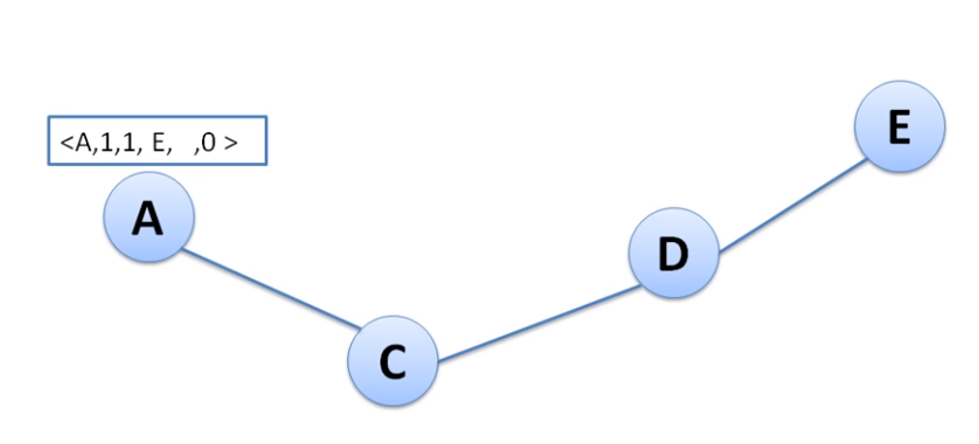
\includegraphics[width=9cm]{gen_route_request}
\caption{生成路由请求}
\end{figure}

\subsubsection{处理和转发路由请求}
一个发起节点总是想和目的节点建立双向的通信,即仅仅是有发起节点有到目的节点的路由还不够,目的节点还必须拥有回到发起节点的路由。因而当RREQ从一个源节点转发到不同的目的节点时,沿途所经过的节点都要自动建立到源节点的反向路由。

节点通过记录收到的第一个RREQ的邻居节点的地址来建立反向路由,或更新原有路由(即更新反向路由表),这些反向路由将会维持一定时间,该段时间足够RREQ在网络内进行转发以及产生的RREP返回源节点。

同时会检查在PATH\_DISCOVERY\_TIME时间内是否受到过具有相同Originator IP Address和RREQ ID的RREQ消息。如果已经接收过了,那么这个节点就会丢弃这个RREQ,不作任何操作。当RREQ到达了目的节点,目的节点就会产生RREP,并利用建立的反向路由来转发RREP。

在转发RREQ前,需要对其进行更新,RREQ消息内的跳数会加一,表明该RREQ又跳过了一个中间节点;Originator Sequence Number(发起节点序列号)会被用来和反向路由里对应的目的节点序列号比较,如果比已经在路由表里的那个大,那么就会被复制到路由表里面。

\begin{figure}[htb]
\centering
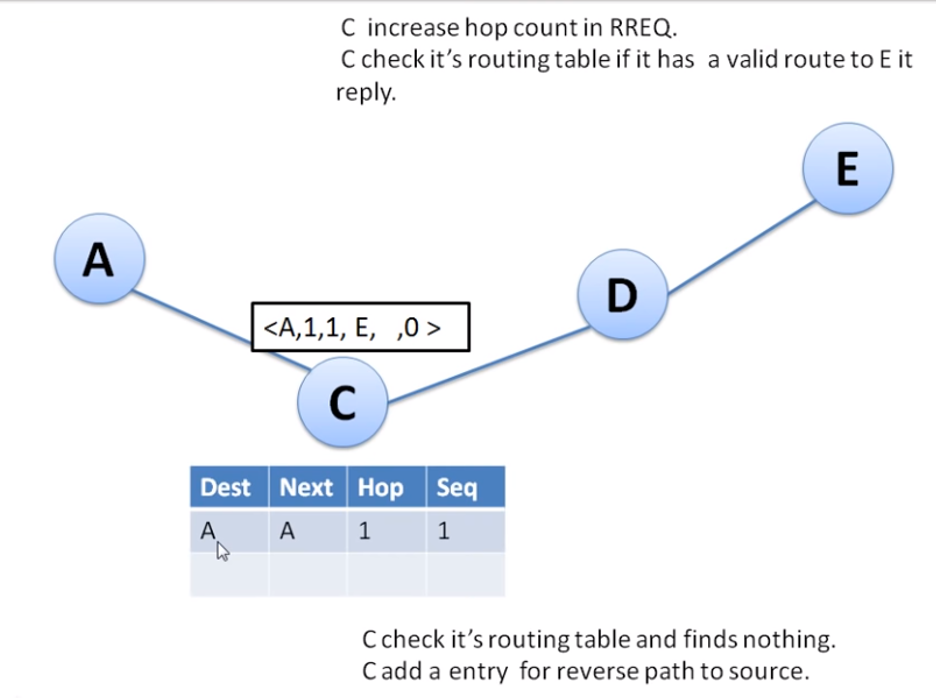
\includegraphics[width=9cm]{handle_route_request_1}
\caption{生成路由请求}
\end{figure}

\begin{figure}[htb]
\centering
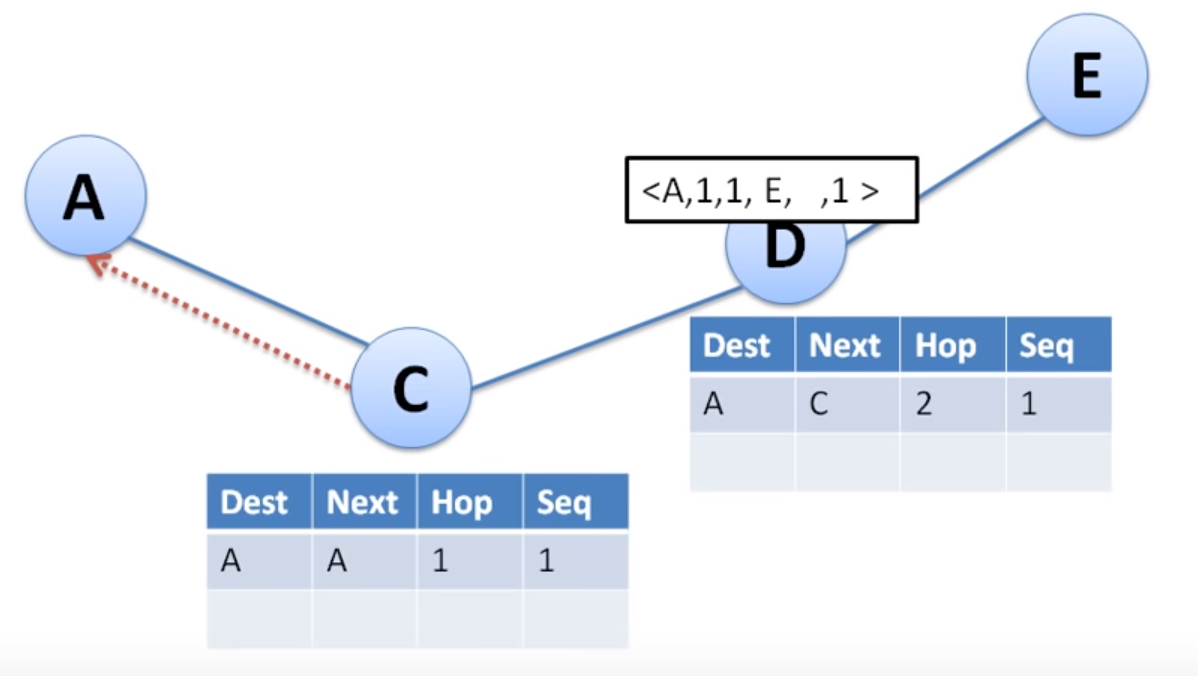
\includegraphics[width=9cm]{handle_route_request_2}
\caption{生成路由请求}
\end{figure}

\subsubsection{生成路由回复}
一个节点在以下情况会生成路由回复消息:
\begin{itemize}
\item 节点本身就是目标节点。
\item 节点存在到目的节点的一条有效路由,且路由表项内的目的节点序列号有效并且不小于RREQ消息内的目的节点序列号
\end{itemize}

RREP一旦被创建,RREP消息就将被送往通向发起节点的下一跳节点,这个节点由路由表里通向发起节点的路由表项给出。当RREP被转发回发起节点时,“跳数”每一跳都会加一,因此当RREP到达发起节点时,这个跳数应当和发起节点到目的节点的跳数一致。

\subsubsection{接受和转发路由回复}
当一个节点收到RREP消息,它将搜索(使用最长前缀匹配)到前一跳的路由;在RREP转发回源节点的过程中,沿着这条路径上的每一个节点都将建立到目的节点的同向路由,即在路由表中记录下RREP是从哪一个邻居节点传来,然后更新有关源和目的路由的时间信息并记录下RREP中目的节点的最新序列号。对于那些建立了反向路由,但RREP并没有经过的节点,它们建立的反向路由将会在一定时间(Active-Route-Timeout)后自动变为无效。

收到RREP的节点将会对到源节点的第一个RREP进行转发,对于其后收到的到同源的RREP,只有当后到的RREP中具有更高的目的序列号或目的序列号相同但所经过的跳数较少时,节点才一会重新更新路由信息并将该RREP转发。根据AODV协议的规定,源节点将在收到第一个RREP后,就开始向目的节点发送数据。


\bibliographystyle{IEEEtran}
\bibliography{ref}

\end{document}